\section{Deconvolution}
\subsection{Inverse filter}
The first and most obvious type of deconvolution is using an inverse filter. We have a blurred image $g$, we found an estimation of the psf ($h_e$) in the previous section %TODO ça sera tjs des sections ?
. So we are theoretically ready to find the original image. We had
\begin{equation}
 g =  h*f,
\end{equation}
in frequency domain
\begin{equation}
G = HF. 
\end{equation}

Using $H_e$, the estimated psf in frequency domain, we can get $F_e$ an so $f_e$ by 
\begin{equation}
F_{e} = H_{e}^{-1} G
\end{equation} 

However it's clear that if we add some noise this model doesn't work anymore. Indeed as shown on figure \ref{fig:psfFFT}, $H_e$ has some value near zero. So when we divide $G$ by this, the noise is strongly amplified by the value near zero. This problem explains the results obtained on figure XXX. %TODO  

\begin{figure}
\centering
\missingfigure{T'as oublié de la pusher}
%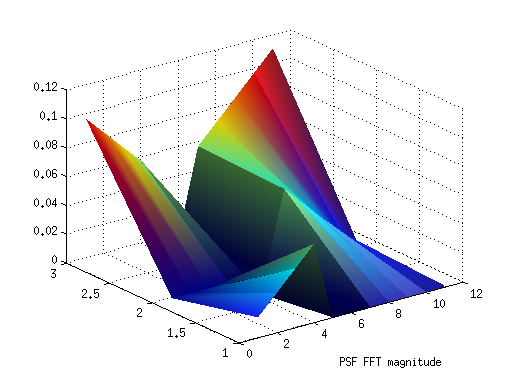
\includegraphics[scale=0.5]{../Images/psfFFT.png}
\caption{FFT of the psf}
\label{fig:psfFFT}
\end{figure}


\subsection{Lucy-Richarson}
\subsubsection{Theory behind the method}
The method was introduced in~\cite{richardson1972bayesian} and
then in~\cite{lucy1974iterative} by Richarson and Lucy respectively.
I these articles, $f$ and $g$ are considered as probability function.
\cite{richardson1972bayesian} says (translated in our notations)
``Units of enery (which may be considered as unique events)
originating at a point in $f$ are distributed at points in $g$
according to the frequencies indicated by $h$''.
However, the justification of~\cite{richardson1972bayesian} (in 1D) uses
$P(f(x)) = \frac{f(x)}{\sum_x f(x)}$ which does not seem
very appropriate.

When \cite{richardson1972bayesian} talks about energy,
that refers to the light which is quantized with photons.
That quantization gives us a reason to model the noise with
poisson distribution.
This modelization of the noise is called the shot noise and
is developped in~\cite{blanter2000shot}.
This model of the noise is used by~\cite{hebert1989generalized}.
\cite{temerinac2010tile} base on~\cite{hebert1989generalized}
and this model of the noise to show (even in 3D)
that the Lucy-Richardson algorithm gives the MLE of $f$ of this
model.

They suggest that $G \sim \pois(h * f)$ ($G$ is capitilize sinced it is a random function).
Therefore,
\begin{align*}
  L(f) & = P(g|f)\\
  & = \prod_{(x,y)} \frac{[(h*f)(x,y)]^{g(x,y)} \exp(-(h*f)(x,y))}{(g(x,y))!}\\
  l(f) & = \sum_{(x,y)} g(x,y)\log((h*f)(x,y)) - (h*f)(x,y) -\log(g(x,y)!).
\end{align*}
Let's first develop
\begin{align*}
  \fpart{(h*g)(x,y)}{f(a,b)} & = \fpart{}{f(a,b)}\sum_{(i,j)}f(i,j)h(x-i,y-j)\\
  \fpart{(h*g)(x,y)}{f(a,b)} & = h(x-a,y-b).
\end{align*}
Consequently, we have
\begin{align*}
  \fpart{l(f)}{f(a,b)} & = \sum_{(x,y)} \left(\frac{g(x,y)}{(h*f)(x,y)} - 1\right) \fpart{(h*g)(x,y)}{f(a,b)}\\
  & = \sum_{(x,y)} \left(\frac{g(x,y)}{(h*f)(x,y)} - 1\right) h(x-a,y-b)\\
  & = \left(\left(\frac{g(x,y)}{(h*f)(x,y)} - 1\right) * h(-x,-y)\right)(a,b)\\
  & = \left(\left(\frac{g(x,y)}{(h*f)(x,y)}\right) * h(-x,-y)\right)(a,b) - 1 * h(-x,-y)\\
  & = \left(\left(\frac{g(x,y)}{(h*f)(x,y)}\right) * h(-x,-y)\right)(a,b) - \left(\sum_{(i,j)} h(-x-i,-y-j)\right)(a,b).
\end{align*}
As explained in the mathematical model,
\[ \sum_{(i,j)} h(i,j) = 1 \]
so we have
\[ \nabla l(f) = \frac{g(x,y)}{(h*f)(x,y)} * h(-x,-y) - 1. \]
To get the minimum of $l(f)$, $\nabla l(f)$ needs to be 0.
Therefore % TODO Justify hessienne
\[ \frac{g(x,y)}{(h*\hat{f})(x,y)} * h(-x,-y) = 1. \]
If we multiply each side by $f(x,y)$, we get
\[ f(x,y)\left(\frac{g(x,y)}{(h*\hat{f})(x,y)} * h(-x,-y)\right) = f(x,y) \]
which can be solved iteratively using the fixed point method which gives us
\[ f_{k+1}(x,y) = f_k(x,y)\left(\frac{g(x,y)}{(h*f_k)(x,y)} * h(-x,-y)\right). \]

\section{Wiener Deconvolution}
 Another deconvolution is the wiener one. 




\section{Regularisation}
%TODO
The last deconvolution method is the deconvolution using regularized filter. 
Instead of a simple inverse 
\begin{equation}
\sum_{m,n} \left[ (g(m,n) - h(m,n)*f(m,n))^2 + \alpha (l(m,n)*f(m,n))^2 \right]
\end{equation}

\begin{equation}
\sum_{k,l} \{ [G(k,l) - H(k,l)F(k,l)]^2 + \alpha [L(k,l)F(k,l)]^2\}
\end{equation}


\begin{equation}
\hat{F}(k,l) = \frac{H(k,l)}{|H(k,l)|^2 + \alpha |L(k,l)|^2} G(k,l)
\end{equation}
